\chapter{Luồng và lát cắt (Flows and cuts)}

Trong chương này, chúng ta tập trung vào hai
bài toán sau:

\begin{itemize}
\item \key{Finding a maximum flow}:
Lượng luồng tối đa chúng ta có thể
gửi từ một nút đến một nút khác là bao nhiêu?
\item \key{Finding a minimum cut}:
Tập hợp các cạnh có trọng số tối thiểu
để tách hai nút của đồ thị là gì?
\end{itemize}

Đầu vào cho cả hai bài toán này là một đồ thị có hướng,
có trọng số, chứa hai nút đặc biệt:
\emph{nguồn (source)} là một nút không có cạnh đi vào,
và \emph{đích (sink)} là một nút không có cạnh đi ra.

Ví dụ, chúng ta sẽ sử dụng đồ thị sau
trong đó nút 1 là nguồn và nút 6
là đích:

\begin{center}
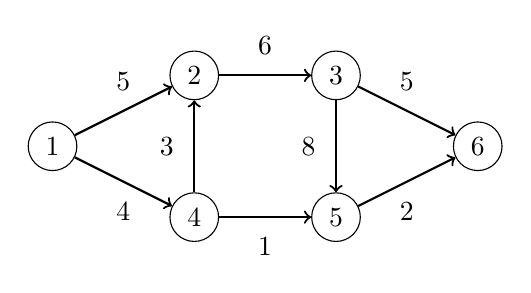
\begin{tikzpicture}[scale=0.9]
\node[draw, circle] (1) at (1,2) {$1$};
\node[draw, circle] (2) at (3,3) {$2$};
\node[draw, circle] (3) at (5,3) {$3$};
\node[draw, circle] (4) at (7,2) {$6$};
\node[draw, circle] (5) at (3,1) {$4$};
\node[draw, circle] (6) at (5,1) {$5$};
\path[draw,thick,->] (1) -- node[font=\small,label=5] {} (2);
\path[draw,thick,->] (2) -- node[font=\small,label=6] {} (3);
\path[draw,thick,->] (3) -- node[font=\small,label=5] {} (4);
\path[draw,thick,->] (1) -- node[font=\small,label=below:4] {} (5);
\path[draw,thick,->] (5) -- node[font=\small,label=below:1] {} (6);
\path[draw,thick,->] (6) -- node[font=\small,label=below:2] {} (4);
\path[draw,thick,<-] (2) -- node[font=\small,label=left:3] {} (5);
\path[draw,thick,->] (3) -- node[font=\small,label=left:8] {} (6);
\end{tikzpicture}
\end{center}

\subsubsection{Maximum flow}

\index{flow}
\index{maximum flow}

Trong bài toán \key{maximum flow},
nhiệm vụ của chúng ta là gửi càng nhiều luồng càng tốt
từ nguồn đến đích.
Trọng số của mỗi cạnh là một sức chứa (capacity)
giới hạn luồng
có thể đi qua cạnh đó.
Ở mỗi nút trung gian,
luồng đi vào và luồng đi ra
phải bằng nhau.

Ví dụ, kích thước tối đa của một luồng
trong đồ thị ví dụ là 7.
Hình sau cho thấy cách chúng ta có thể
định tuyến luồng:

\begin{center}
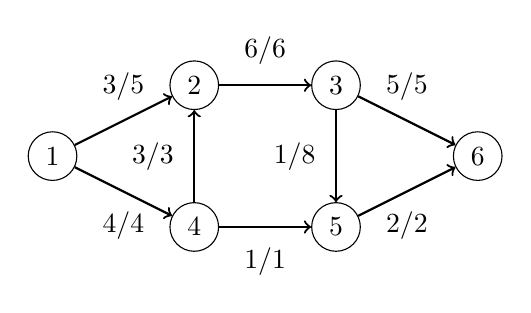
\begin{tikzpicture}[scale=0.9]
\node[draw, circle] (1) at (1,2) {$1$};
\node[draw, circle] (2) at (3,3) {$2$};
\node[draw, circle] (3) at (5,3) {$3$};
\node[draw, circle] (4) at (7,2) {$6$};
\node[draw, circle] (5) at (3,1) {$4$};
\node[draw, circle] (6) at (5,1) {$5$};
\path[draw,thick,->] (1) -- node[font=\small,label=3/5] {} (2);
\path[draw,thick,->] (2) -- node[font=\small,label=6/6] {} (3);
\path[draw,thick,->] (3) -- node[font=\small,label=5/5] {} (4);
\path[draw,thick,->] (1) -- node[font=\small,label=below:4/4] {} (5);
\path[draw,thick,->] (5) -- node[font=\small,label=below:1/1] {} (6);
\path[draw,thick,->] (6) -- node[font=\small,label=below:2/2] {} (4);
\path[draw,thick,<-] (2) -- node[font=\small,label=left:3/3] {} (5);
\path[draw,thick,->] (3) -- node[font=\small,label=left:1/8] {} (6);
\end{tikzpicture}
\end{center}

Ký hiệu $v/k$ có nghĩa là
một luồng $v$ đơn vị được định tuyến qua
một cạnh có sức chứa là $k$ đơn vị.
Kích thước của luồng là $7$,
bởi vì nguồn gửi đi $3+4$ đơn vị luồng
và đích nhận $5+2$ đơn vị luồng.
Dễ thấy luồng này là cực đại,
bởi vì tổng sức chứa của các cạnh
dẫn đến đích là $7$.

\subsubsection{Minimum cut}

\index{cut}
\index{minimum cut}

Trong bài toán \key{minimum cut},
nhiệm vụ của chúng ta là loại bỏ một tập hợp
các cạnh khỏi đồ thị
sao cho không còn đường đi từ nguồn
đến đích sau khi loại bỏ
và tổng trọng số của các cạnh bị loại bỏ
là tối thiểu.

Kích thước tối thiểu của một lát cắt trong đồ thị ví dụ là 7.
Chỉ cần loại bỏ các cạnh $2 \rightarrow 3$
và $4 \rightarrow 5$:

\begin{center}
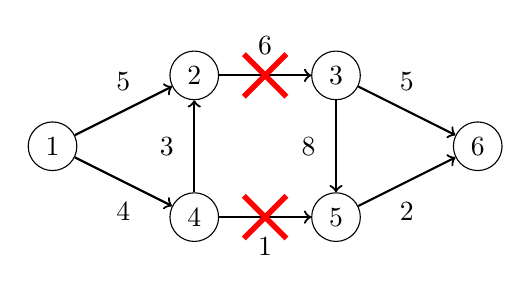
\begin{tikzpicture}[scale=0.9]
\node[draw, circle] (1) at (1,2) {$1$};
\node[draw, circle] (2) at (3,3) {$2$};
\node[draw, circle] (3) at (5,3) {$3$};
\node[draw, circle] (4) at (7,2) {$6$};
\node[draw, circle] (5) at (3,1) {$4$};
\node[draw, circle] (6) at (5,1) {$5$};
\path[draw,thick,->] (1) -- node[font=\small,label=5] {} (2);
\path[draw,thick,->] (2) -- node[font=\small,label=6] {} (3);
\path[draw,thick,->] (3) -- node[font=\small,label=5] {} (4);
\path[draw,thick,->] (1) -- node[font=\small,label=below:4] {} (5);
\path[draw,thick,->] (5) -- node[font=\small,label=below:1] {} (6);
\path[draw,thick,->] (6) -- node[font=\small,label=below:2] {} (4);
\path[draw,thick,<-] (2) -- node[font=\small,label=left:3] {} (5);
\path[draw,thick,->] (3) -- node[font=\small,label=left:8] {} (6);

\path[draw=red,thick,-,line width=2pt] (4-.3,3-.3) -- (4+.3,3+.3);
\path[draw=red,thick,-,line width=2pt] (4-.3,3+.3) -- (4+.3,3-.3);
\path[draw=red,thick,-,line width=2pt] (4-.3,1-.3) -- (4+.3,1+.3);
\path[draw=red,thick,-,line width=2pt] (4-.3,1+.3) -- (4+.3,1-.3);
\end{tikzpicture}
\end{center}

Sau khi loại bỏ các cạnh,
sẽ không còn đường đi nào từ nguồn đến đích.
Kích thước của lát cắt là $7$,
bởi vì trọng số của các cạnh bị loại bỏ
là $6$ và $1$.
Lát cắt này là tối thiểu, vì không có
cách hợp lệ nào để loại bỏ các cạnh khỏi đồ thị sao cho
tổng trọng số của chúng nhỏ hơn $7$.
\\\\
Không phải ngẫu nhiên mà
kích thước tối đa của một luồng
và kích thước tối thiểu của một lát cắt
lại bằng nhau trong ví dụ trên.
Hóa ra luồng cực đại
và lát cắt cực tiểu
\emph{luôn luôn} có độ lớn bằng nhau,
vì vậy các khái niệm này là hai mặt của cùng một đồng xu.

Tiếp theo chúng ta sẽ thảo luận về thuật toán Ford–Fulkerson
có thể được sử dụng để tìm
luồng cực đại và lát cắt cực tiểu của một đồ thị.
Thuật toán này cũng giúp chúng ta hiểu
\emph{tại sao} chúng lại có độ lớn bằng nhau.

\section{Thuật toán Ford–Fulkerson}

\index{Ford–Fulkerson algorithm}

\key{Thuật toán Ford–Fulkerson (Ford–Fulkerson algorithm)} \cite{for56} tìm
luồng cực đại trong một đồ thị.
Thuật toán bắt đầu với một luồng rỗng,
và ở mỗi bước tìm một đường đi từ nguồn
đến đích để tạo ra nhiều luồng hơn.
Cuối cùng, khi thuật toán không thể tăng luồng
được nữa, luồng cực đại đã được tìm thấy.

Thuật toán sử dụng một biểu diễn đặc biệt
của đồ thị, trong đó mỗi cạnh ban đầu có một cạnh ngược
theo hướng khác.
Trọng số của mỗi cạnh cho biết chúng ta
có thể định tuyến thêm bao nhiêu luồng qua nó.
Khi bắt đầu thuật toán, trọng số của mỗi cạnh ban đầu
bằng sức chứa của cạnh đó
và trọng số của mỗi cạnh ngược là không.

\begin{samepage}
Biểu diễn mới cho đồ thị ví dụ như sau:

\begin{center}
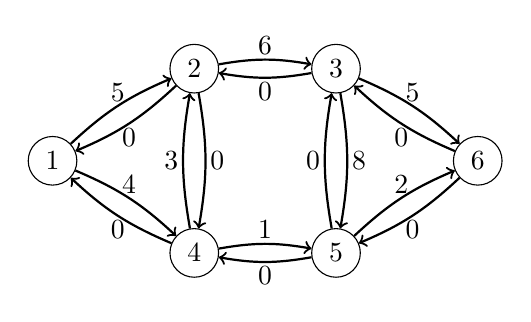
\begin{tikzpicture}[scale=0.9,label distance=-2mm]
\node[draw, circle] (1) at (1,1.3) {$1$};
\node[draw, circle] (2) at (3,2.6) {$2$};
\node[draw, circle] (3) at (5,2.6) {$3$};
\node[draw, circle] (4) at (7,1.3) {$6$};
\node[draw, circle] (5) at (3,0) {$4$};
\node[draw, circle] (6) at (5,0) {$5$};

\path[draw,thick,->] (1) edge [bend left=10] node[font=\small,label=5] {} (2);
\path[draw,thick,->] (2) edge [bend left=10] node[font=\small,label=below:0] {} (1);
\path[draw,thick,->] (2) edge [bend left=10] node[font=\small,label=6] {} (3);
\path[draw,thick,->] (3) edge [bend left=10] node[font=\small,label=below:0] {} (2);
\path[draw,thick,->] (3) edge [bend left=10] node[font=\small,label=5] {} (4);
\path[draw,thick,->] (4) edge [bend left=10] node[font=\small,label=below:0] {} (3);
\path[draw,thick,->] (1) edge [bend left=10] node[font=\small,label=4] {} (5);
\path[draw,thick,->] (5) edge [bend left=10] node[font=\small,label=below:0] {} (1);
\path[draw,thick,->] (5) edge [bend left=10] node[font=\small,label=1] {} (6);
\path[draw,thick,->] (6) edge [bend left=10] node[font=\small,label=below:0] {} (5);
\path[draw,thick,->] (6) edge [bend left=10] node[font=\small,label=2] {} (4);
\path[draw,thick,->] (4) edge [bend left=10] node[font=\small,label=below:0] {} (6);
\path[draw,thick,->] (5) edge [bend left=10] node[font=\small,label=left:3] {} (2);
\path[draw,thick,->] (2) edge [bend left=10] node[font=\small,label=right:0] {} (5);
\path[draw,thick,->] (3) edge [bend left=10] node[font=\small,label=right:8] {} (6);
\path[draw,thick,->] (6) edge [bend left=10] node[font=\small,label=left:0] {} (3);
\end{tikzpicture}
\end{center}
\end{samepage}

\subsubsection{Mô tả thuật toán}

Thuật toán Ford–Fulkerson bao gồm nhiều
vòng.
Ở mỗi vòng, thuật toán tìm
một đường đi từ nguồn đến đích
sao cho mỗi cạnh trên đường đi có trọng số dương.
Nếu có nhiều hơn một đường đi khả dụng,
chúng ta có thể chọn bất kỳ đường nào trong số đó.

Ví dụ, giả sử chúng ta chọn đường đi sau:

\begin{center}
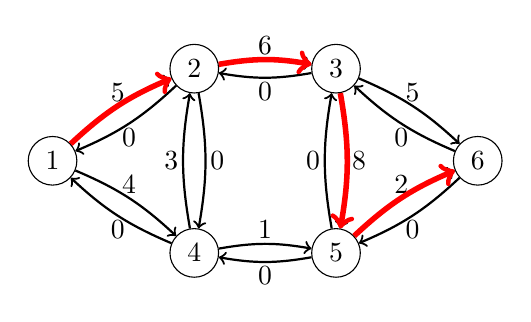
\begin{tikzpicture}[scale=0.9,label distance=-2mm]
\node[draw, circle] (1) at (1,1.3) {$1$};
\node[draw, circle] (2) at (3,2.6) {$2$};
\node[draw, circle] (3) at (5,2.6) {$3$};
\node[draw, circle] (4) at (7,1.3) {$6$};
\node[draw, circle] (5) at (3,0) {$4$};
\node[draw, circle] (6) at (5,0) {$5$};

\path[draw,thick,->] (1) edge [bend left=10] node[font=\small,label=5] {} (2);
\path[draw,thick,->] (2) edge [bend left=10] node[font=\small,label=below:0] {} (1);
\path[draw,thick,->] (2) edge [bend left=10] node[font=\small,label=6] {} (3);
\path[draw,thick,->] (3) edge [bend left=10] node[font=\small,label=below:0] {} (2);
\path[draw,thick,->] (3) edge [bend left=10] node[font=\small,label=5] {} (4);
\path[draw,thick,->] (4) edge [bend left=10] node[font=\small,label=below:0] {} (3);
\path[draw,thick,->] (1) edge [bend left=10] node[font=\small,label=4] {} (5);
\path[draw,thick,->] (5) edge [bend left=10] node[font=\small,label=below:0] {} (1);
\path[draw,thick,->] (5) edge [bend left=10] node[font=\small,label=1] {} (6);
\path[draw,thick,->] (6) edge [bend left=10] node[font=\small,label=below:0] {} (5);
\path[draw,thick,->] (6) edge [bend left=10] node[font=\small,label=2] {} (4);
\path[draw,thick,->] (4) edge [bend left=10] node[font=\small,label=below:0] {} (6);
\path[draw,thick,->] (5) edge [bend left=10] node[font=\small,label=left:3] {} (2);
\path[draw,thick,->] (2) edge [bend left=10] node[font=\small,label=right:0] {} (5);
\path[draw,thick,->] (3) edge [bend left=10] node[font=\small,label=right:8] {} (6);
\path[draw,thick,->] (6) edge [bend left=10] node[font=\small,label=left:0] {} (3);

\path[draw=red,thick,->,line width=2pt] (1) edge [bend left=10] (2);
\path[draw=red,thick,->,line width=2pt] (2) edge [bend left=10] (3);
\path[draw=red,thick,->,line width=2pt] (3) edge [bend left=10] (6);
\path[draw=red,thick,->,line width=2pt] (6) edge [bend left=10] (4);
\end{tikzpicture}
\end{center}

Sau khi chọn đường đi, luồng tăng thêm $x$ đơn vị,
trong đó $x$ là trọng số cạnh nhỏ nhất trên đường đi.
Ngoài ra, trọng số của mỗi cạnh trên đường đi
giảm đi $x$ và trọng số của mỗi cạnh ngược
tăng thêm $x$.

Trong đường đi trên, trọng số của các
cạnh là 5, 6, 8 và 2.
Trọng số nhỏ nhất là 2,
vì vậy luồng tăng thêm 2
và đồ thị mới như sau:

\begin{center}
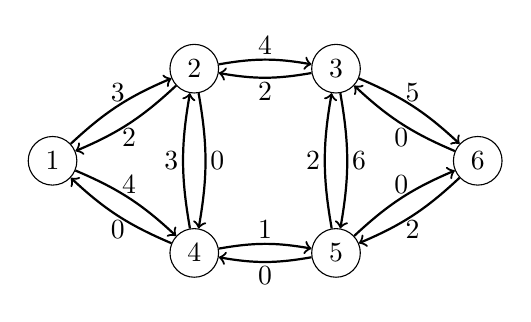
\begin{tikzpicture}[scale=0.9,label distance=-2mm]
\node[draw, circle] (1) at (1,1.3) {$1$};
\node[draw, circle] (2) at (3,2.6) {$2$};
\node[draw, circle] (3) at (5,2.6) {$3$};
\node[draw, circle] (4) at (7,1.3) {$6$};
\node[draw, circle] (5) at (3,0) {$4$};
\node[draw, circle] (6) at (5,0) {$5$};

\path[draw,thick,->] (1) edge [bend left=10] node[font=\small,label=3] {} (2);
\path[draw,thick,->] (2) edge [bend left=10] node[font=\small,label=below:2] {} (1);
\path[draw,thick,->] (2) edge [bend left=10] node[font=\small,label=4] {} (3);
\path[draw,thick,->] (3) edge [bend left=10] node[font=\small,label=below:2] {} (2);
\path[draw,thick,->] (3) edge [bend left=10] node[font=\small,label=5] {} (4);
\path[draw,thick,->] (4) edge [bend left=10] node[font=\small,label=below:0] {} (3);
\path[draw,thick,->] (1) edge [bend left=10] node[font=\small,label=4] {} (5);
\path[draw,thick,->] (5) edge [bend left=10] node[font=\small,label=below:0] {} (1);
\path[draw,thick,->] (5) edge [bend left=10] node[font=\small,label=1] {} (6);
\path[draw,thick,->] (6) edge [bend left=10] node[font=\small,label=below:0] {} (5);
\path[draw,thick,->] (6) edge [bend left=10] node[font=\small,label=0] {} (4);
\path[draw,thick,->] (4) edge [bend left=10] node[font=\small,label=below:2] {} (6);
\path[draw,thick,->] (5) edge [bend left=10] node[font=\small,label=left:3] {} (2);
\path[draw,thick,->] (2) edge [bend left=10] node[font=\small,label=right:0] {} (5);
\path[draw,thick,->] (3) edge [bend left=10] node[font=\small,label=right:6] {} (6);
\path[draw,thick,->] (6) edge [bend left=10] node[font=\small,label=left:2] {} (3);
\end{tikzpicture}
\end{center}

Ý tưởng là việc tăng luồng sẽ làm giảm lượng
luồng có thể đi qua các cạnh trong tương lai.
Mặt khác, có thể hủy
luồng sau này bằng cách sử dụng các cạnh ngược của đồ thị
nếu hóa ra việc
định tuyến luồng theo một cách khác sẽ có lợi hơn.

Thuật toán tăng luồng miễn là
còn một đường đi từ nguồn
đến đích qua các cạnh có trọng số dương.
Trong ví dụ hiện tại, đường đi tiếp theo của chúng ta có thể như sau:

\begin{center}
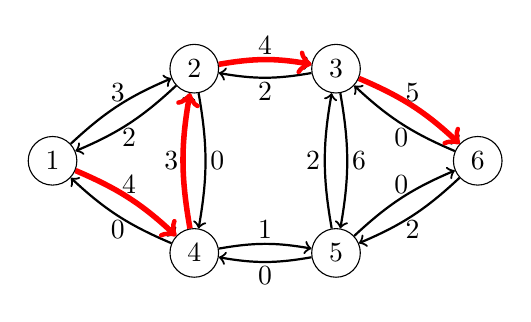
\begin{tikzpicture}[scale=0.9,label distance=-2mm]
\node[draw, circle] (1) at (1,1.3) {$1$};
\node[draw, circle] (2) at (3,2.6) {$2$};
\node[draw, circle] (3) at (5,2.6) {$3$};
\node[draw, circle] (4) at (7,1.3) {$6$};
\node[draw, circle] (5) at (3,0) {$4$};
\node[draw, circle] (6) at (5,0) {$5$};

\path[draw,thick,->] (1) edge [bend left=10] node[font=\small,label=3] {} (2);
\path[draw,thick,->] (2) edge [bend left=10] node[font=\small,label=below:2] {} (1);
\path[draw,thick,->] (2) edge [bend left=10] node[font=\small,label=4] {} (3);
\path[draw,thick,->] (3) edge [bend left=10] node[font=\small,label=below:2] {} (2);
\path[draw,thick,->] (3) edge [bend left=10] node[font=\small,label=5] {} (4);
\path[draw,thick,->] (4) edge [bend left=10] node[font=\small,label=below:0] {} (3);
\path[draw,thick,->] (1) edge [bend left=10] node[font=\small,label=4] {} (5);
\path[draw,thick,->] (5) edge [bend left=10] node[font=\small,label=below:0] {} (1);
\path[draw,thick,->] (5) edge [bend left=10] node[font=\small,label=1] {} (6);
\path[draw,thick,->] (6) edge [bend left=10] node[font=\small,label=below:0] {} (5);
\path[draw,thick,->] (6) edge [bend left=10] node[font=\small,label=0] {} (4);
\path[draw,thick,->] (4) edge [bend left=10] node[font=\small,label=below:2] {} (6);
\path[draw,thick,->] (5) edge [bend left=10] node[font=\small,label=left:3] {} (2);
\path[draw,thick,->] (2) edge [bend left=10] node[font=\small,label=right:0] {} (5);
\path[draw,thick,->] (3) edge [bend left=10] node[font=\small,label=right:6] {} (6);
\path[draw,thick,->] (6) edge [bend left=10] node[font=\small,label=left:2] {} (3);

\path[draw=red,thick,->,line width=2pt] (1) edge [bend left=10] (5);
\path[draw=red,thick,->,line width=2pt] (5) edge [bend left=10] (2);
\path[draw=red,thick,->,line width=2pt] (2) edge [bend left=10] (3);
\path[draw=red,thick,->,line width=2pt] (3) edge [bend left=10] (4);
\end{tikzpicture}
\end{center}

Trọng số cạnh nhỏ nhất trên đường đi này là 3,
vì vậy đường đi này tăng luồng thêm 3,
và tổng luồng sau khi xử lý đường đi là 5.

\begin{samepage}
Đồ thị mới sẽ như sau:

\begin{center}
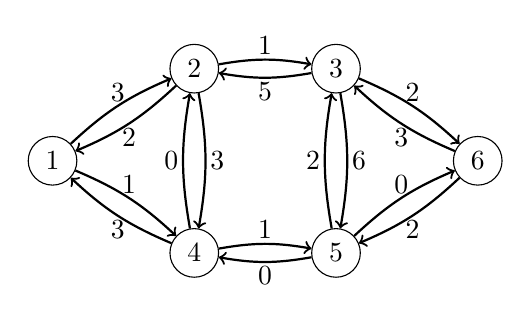
\begin{tikzpicture}[scale=0.9,label distance=-2mm]
\node[draw, circle] (1) at (1,1.3) {$1$};
\node[draw, circle] (2) at (3,2.6) {$2$};
\node[draw, circle] (3) at (5,2.6) {$3$};
\node[draw, circle] (4) at (7,1.3) {$6$};
\node[draw, circle] (5) at (3,0) {$4$};
\node[draw, circle] (6) at (5,0) {$5$};

\path[draw,thick,->] (1) edge [bend left=10] node[font=\small,label=3] {} (2);
\path[draw,thick,->] (2) edge [bend left=10] node[font=\small,label=below:2] {} (1);
\path[draw,thick,->] (2) edge [bend left=10] node[font=\small,label=1] {} (3);
\path[draw,thick,->] (3) edge [bend left=10] node[font=\small,label=below:5] {} (2);
\path[draw,thick,->] (3) edge [bend left=10] node[font=\small,label=2] {} (4);
\path[draw,thick,->] (4) edge [bend left=10] node[font=\small,label=below:3] {} (3);
\path[draw,thick,->] (1) edge [bend left=10] node[font=\small,label=1] {} (5);
\path[draw,thick,->] (5) edge [bend left=10] node[font=\small,label=below:3] {} (1);
\path[draw,thick,->] (5) edge [bend left=10] node[font=\small,label=1] {} (6);
\path[draw,thick,->] (6) edge [bend left=10] node[font=\small,label=below:0] {} (5);
\path[draw,thick,->] (6) edge [bend left=10] node[font=\small,label=0] {} (4);
\path[draw,thick,->] (4) edge [bend left=10] node[font=\small,label=below:2] {} (6);
\path[draw,thick,->] (5) edge [bend left=10] node[font=\small,label=left:0] {} (2);
\path[draw,thick,->] (2) edge [bend left=10] node[font=\small,label=right:3] {} (5);
\path[draw,thick,->] (3) edge [bend left=10] node[font=\small,label=right:6] {} (6);
\path[draw,thick,->] (6) edge [bend left=10] node[font=\small,label=left:2] {} (3);
\end{tikzpicture}
\end{center}
\end{samepage}

Chúng ta vẫn cần thêm hai vòng nữa trước khi đạt được luồng cực đại.
Ví dụ, chúng ta có thể chọn các đường đi
$1 \rightarrow 2 \rightarrow 3 \rightarrow 6$ và
$1 \rightarrow 4 \rightarrow 5 \rightarrow 3 \rightarrow 6$.
Cả hai đường đi đều tăng luồng thêm 1,
và đồ thị cuối cùng như sau:

\begin{center}
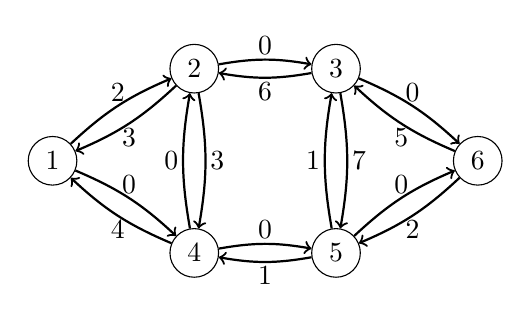
\begin{tikzpicture}[scale=0.9,label distance=-2mm]
\node[draw, circle] (1) at (1,1.3) {$1$};
\node[draw, circle] (2) at (3,2.6) {$2$};
\node[draw, circle] (3) at (5,2.6) {$3$};
\node[draw, circle] (4) at (7,1.3) {$6$};
\node[draw, circle] (5) at (3,0) {$4$};
\node[draw, circle] (6) at (5,0) {$5$};

\path[draw,thick,->] (1) edge [bend left=10] node[font=\small,label=2] {} (2);
\path[draw,thick,->] (2) edge [bend left=10] node[font=\small,label=below:3] {} (1);
\path[draw,thick,->] (2) edge [bend left=10] node[font=\small,label=0] {} (3);
\path[draw,thick,->] (3) edge [bend left=10] node[font=\small,label=below:6] {} (2);
\path[draw,thick,->] (3) edge [bend left=10] node[font=\small,label=0] {} (4);
\path[draw,thick,->] (4) edge [bend left=10] node[font=\small,label=below:5] {} (3);
\path[draw,thick,->] (1) edge [bend left=10] node[font=\small,label=0] {} (5);
\path[draw,thick,->] (5) edge [bend left=10] node[font=\small,label=below:4] {} (1);
\path[draw,thick,->] (5) edge [bend left=10] node[font=\small,label=0] {} (6);
\path[draw,thick,->] (6) edge [bend left=10] node[font=\small,label=below:1] {} (5);
\path[draw,thick,->] (6) edge [bend left=10] node[font=\small,label=0] {} (4);
\path[draw,thick,->] (4) edge [bend left=10] node[font=\small,label=below:2] {} (6);
\path[draw,thick,->] (5) edge [bend left=10] node[font=\small,label=left:0] {} (2);
\path[draw,thick,->] (2) edge [bend left=10] node[font=\small,label=right:3] {} (5);
\path[draw,thick,->] (3) edge [bend left=10] node[font=\small,label=right:7] {} (6);
\path[draw,thick,->] (6) edge [bend left=10] node[font=\small,label=left:1] {} (3);
\end{tikzpicture}
\end{center}

Không thể tăng luồng thêm nữa,
vì không còn đường đi nào từ nguồn
đến đích có trọng số cạnh dương.
Do đó, thuật toán kết thúc và luồng cực đại là 7.

\subsubsection{Tìm đường đi}

Thuật toán Ford–Fulkerson không chỉ định
cách chúng ta nên chọn các đường đi để tăng luồng.
Trong mọi trường hợp, thuật toán sẽ kết thúc sớm hay muộn
và tìm đúng luồng cực đại.
Tuy nhiên, hiệu quả của thuật toán phụ thuộc vào
cách các đường đi được chọn.

Một cách đơn giản để tìm đường đi là sử dụng tìm kiếm theo chiều sâu.
Thông thường, cách này hoạt động tốt, nhưng trong trường hợp xấu nhất,
mỗi đường đi chỉ tăng luồng thêm 1
và thuật toán sẽ chậm.
May mắn thay, chúng ta có thể tránh tình huống này
bằng cách sử dụng một trong các kỹ thuật sau:

\index{Edmonds–Karp algorithm}

\key{Thuật toán Edmonds–Karp (Edmonds–Karp algorithm)} \cite{edm72}
chọn mỗi đường đi sao cho số lượng cạnh
trên đường đi là nhỏ nhất có thể.
Điều này có thể được thực hiện bằng cách sử dụng tìm kiếm theo chiều rộng
thay vì tìm kiếm theo chiều sâu để tìm đường đi.
Có thể chứng minh rằng điều này đảm bảo
luồng tăng nhanh, và độ phức tạp thời gian
của thuật toán là $O(m^2 n)$.

\index{scaling algorithm}

\key{Thuật toán co giãn (scaling algorithm)} \cite{ahu91} sử dụng tìm kiếm theo chiều sâu
để tìm các đường đi trong đó mỗi trọng số cạnh
ít nhất bằng một giá trị ngưỡng.
Ban đầu, giá trị ngưỡng là
một số lớn nào đó, ví dụ như tổng tất cả
trọng số cạnh của đồ thị.
Mỗi khi không tìm thấy đường đi,
giá trị ngưỡng được chia cho 2.
Độ phức tạp thời gian của thuật toán là $O(m^2 \log c)$,
trong đó $c$ là giá trị ngưỡng ban đầu.

Trong thực tế, thuật toán co giãn dễ thực hiện hơn,
vì có thể sử dụng tìm kiếm theo chiều sâu để tìm đường đi.
Cả hai thuật toán đều đủ hiệu quả cho các bài toán
thường xuất hiện trong các cuộc thi lập trình.

\subsubsection{Minimum cuts}

\index{minimum cut}

Hóa ra một khi thuật toán Ford–Fulkerson
đã tìm thấy một luồng cực đại,
nó cũng đã xác định được một lát cắt cực tiểu.
Gọi $A$ là tập hợp các nút
có thể đến được từ nguồn
bằng cách sử dụng các cạnh có trọng số dương.
Trong đồ thị ví dụ, $A$ chứa các nút 1, 2 và 4:

\begin{center}
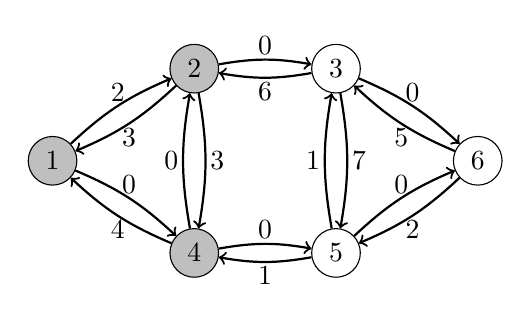
\begin{tikzpicture}[scale=0.9,label distance=-2mm]
\node[draw, circle,fill=lightgray] (1) at (1,1.3) {$1$};
\node[draw, circle,fill=lightgray] (2) at (3,2.6) {$2$};
\node[draw, circle] (3) at (5,2.6) {$3$};
\node[draw, circle] (4) at (7,1.3) {$6$};
\node[draw, circle,fill=lightgray] (5) at (3,0) {$4$};
\node[draw, circle] (6) at (5,0) {$5$};

\path[draw,thick,->] (1) edge [bend left=10] node[font=\small,label=2] {} (2);
\path[draw,thick,->] (2) edge [bend left=10] node[font=\small,label=below:3] {} (1);
\path[draw,thick,->] (2) edge [bend left=10] node[font=\small,label=0] {} (3);
\path[draw,thick,->] (3) edge [bend left=10] node[font=\small,label=below:6] {} (2);
\path[draw,thick,->] (3) edge [bend left=10] node[font=\small,label=0] {} (4);
\path[draw,thick,->] (4) edge [bend left=10] node[font=\small,label=below:5] {} (3);
\path[draw,thick,->] (1) edge [bend left=10] node[font=\small,label=0] {} (5);
\path[draw,thick,->] (5) edge [bend left=10] node[font=\small,label=below:4] {} (1);
\path[draw,thick,->] (5) edge [bend left=10] node[font=\small,label=0] {} (6);
\path[draw,thick,->] (6) edge [bend left=10] node[font=\small,label=below:1] {} (5);
\path[draw,thick,->] (6) edge [bend left=10] node[font=\small,label=0] {} (4);
\path[draw,thick,->] (4) edge [bend left=10] node[font=\small,label=below:2] {} (6);
\path[draw,thick,->] (5) edge [bend left=10] node[font=\small,label=left:0] {} (2);
\path[draw,thick,->] (2) edge [bend left=10] node[font=\small,label=right:3] {} (5);
\path[draw,thick,->] (3) edge [bend left=10] node[font=\small,label=right:7] {} (6);
\path[draw,thick,->] (6) edge [bend left=10] node[font=\small,label=left:1] {} (3);
\end{tikzpicture}
\end{center}

Bây giờ lát cắt cực tiểu bao gồm các cạnh của đồ thị ban đầu
bắt đầu tại một nút nào đó trong $A$, kết thúc tại một nút nào đó bên ngoài $A$,
và có sức chứa được sử dụng
toàn bộ trong luồng cực đại.
Trong đồ thị trên, các cạnh đó là
$2 \rightarrow 3$ và $4 \rightarrow 5$,
tương ứng với lát cắt cực tiểu $6+1=7$.

Tại sao luồng do thuật toán tạo ra là cực đại
và tại sao lát cắt là cực tiểu?
Lý do là một đồ thị không thể
chứa một luồng có kích thước lớn hơn
trọng số của bất kỳ lát cắt nào của đồ thị.
Do đó, bất cứ khi nào một luồng và một lát cắt có độ lớn bằng nhau,
chúng là một luồng cực đại và một lát cắt cực tiểu.

Hãy xem xét bất kỳ lát cắt nào của đồ thị
sao cho nguồn thuộc $A$,
đích thuộc $B$
và có một số cạnh giữa các tập hợp:

\begin{center}
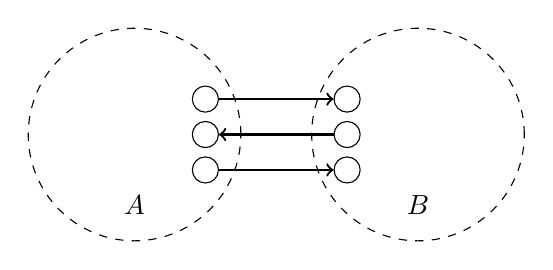
\begin{tikzpicture}[scale=0.9]
\draw[dashed] (-2,0) circle (1.5);
\draw[dashed] (2,0) circle (1.5);

\node at (-2,-1) {$A$};
\node at (2,-1) {$B$};

\node[draw, circle] (1) at (-1,0.5) {};
\node[draw, circle] (2) at (-1,0) {};
\node[draw, circle] (3) at (-1,-0.5) {};
\node[draw, circle] (4) at (1,0.5) {};
\node[draw, circle] (5) at (1,0) {};
\node[draw, circle] (6) at (1,-0.5) {};

\path[draw,thick,->] (1) -- (4);
\path[draw,thick,->] (5) -- (2);
\path[draw,thick,->] (3) -- (6);

\end{tikzpicture}
\end{center}

Kích thước của lát cắt là tổng của các cạnh
đi từ $A$ đến $B$.
Đây là một giới hạn trên cho luồng
trong đồ thị, bởi vì luồng phải đi
từ $A$ đến $B$.
Do đó, kích thước của một luồng cực đại nhỏ hơn hoặc bằng
kích thước của bất kỳ lát cắt nào trong đồ thị.

Mặt khác, thuật toán Ford–Fulkerson
tạo ra một luồng có kích thước \emph{chính xác} bằng
kích thước của một lát cắt trong đồ thị.
Do đó, luồng phải là luồng cực đại
và lát cắt phải là lát cắt cực tiểu.

\section{Đường đi không giao nhau (Disjoint paths)}

Nhiều bài toán đồ thị có thể được giải quyết bằng cách quy
chúng về bài toán luồng cực đại.
Ví dụ đầu tiên của chúng ta về một bài toán như vậy là
như sau: chúng ta được cho một đồ thị có hướng
với một nguồn và một đích,
và nhiệm vụ của chúng ta là tìm số lượng tối đa
các đường đi không giao nhau từ nguồn đến đích.

\subsubsection{Edge-disjoint paths}

Đầu tiên chúng ta sẽ tập trung vào bài toán
tìm số lượng tối đa các
\key{đường đi không giao nhau trên cạnh (edge-disjoint paths)} từ nguồn đến đích.
Điều này có nghĩa là chúng ta nên xây dựng một tập hợp các đường đi
sao cho mỗi cạnh xuất hiện trong tối đa một đường đi.

Ví dụ, hãy xem xét đồ thị sau:
\begin{center}
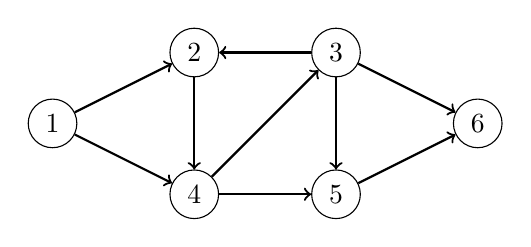
\begin{tikzpicture}[scale=0.9]
\node[draw, circle] (1) at (1,2) {$1$};
\node[draw, circle] (2) at (3,3) {$2$};
\node[draw, circle] (3) at (5,3) {$3$};
\node[draw, circle] (4) at (3,1) {$4$};
\node[draw, circle] (5) at (5,1) {$5$};
\node[draw, circle] (6) at (7,2) {$6$};
\path[draw,thick,->] (1) -- (2);
\path[draw,thick,->] (1) -- (4);
\path[draw,thick,->] (2) -- (4);
\path[draw,thick,->] (3) -- (2);
\path[draw,thick,->] (3) -- (5);
\path[draw,thick,->] (3) -- (6);
\path[draw,thick,->] (4) -- (3);
\path[draw,thick,->] (4) -- (5);
\path[draw,thick,->] (5) -- (6);
\end{tikzpicture}
\end{center}

Trong đồ thị này, số lượng tối đa các đường đi không giao nhau
trên cạnh là 2.
Chúng ta có thể chọn các đường đi
$1 \rightarrow 2 \rightarrow 4 \rightarrow 3 \rightarrow 6$
và $1 \rightarrow 4 \rightarrow 5 \rightarrow 6$ như sau:

\begin{center}
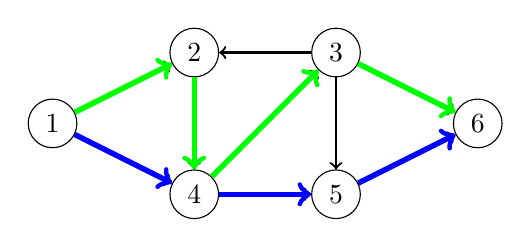
\begin{tikzpicture}[scale=0.9]
\node[draw, circle] (1) at (1,2) {$1$};
\node[draw, circle] (2) at (3,3) {$2$};
\node[draw, circle] (3) at (5,3) {$3$};
\node[draw, circle] (4) at (3,1) {$4$};
\node[draw, circle] (5) at (5,1) {$5$};
\node[draw, circle] (6) at (7,2) {$6$};
\path[draw,thick,->] (1) -- (2);
\path[draw,thick,->] (1) -- (4);
\path[draw,thick,->] (2) -- (4);
\path[draw,thick,->] (3) -- (2);
\path[draw,thick,->] (3) -- (5);
\path[draw,thick,->] (3) -- (6);
\path[draw,thick,->] (4) -- (3);
\path[draw,thick,->] (4) -- (5);
\path[draw,thick,->] (5) -- (6);

\path[draw=green,thick,->,line width=2pt] (1) -- (2);
\path[draw=green,thick,->,line width=2pt] (2) -- (4);
\path[draw=green,thick,->,line width=2pt] (4) -- (3);
\path[draw=green,thick,->,line width=2pt] (3) -- (6);

\path[draw=blue,thick,->,line width=2pt] (1) -- (4);
\path[draw=blue,thick,->,line width=2pt] (4) -- (5);
\path[draw=blue,thick,->,line width=2pt] (5) -- (6);
\end{tikzpicture}
\end{center}

Hóa ra số lượng tối đa các
đường đi không giao nhau trên cạnh
bằng luồng cực đại của đồ thị,
giả sử sức chứa của mỗi cạnh là một.
Sau khi luồng cực đại đã được xây dựng,
các đường đi không giao nhau trên cạnh có thể được tìm thấy một cách tham lam
bằng cách đi theo các đường đi từ nguồn đến đích.

\subsubsection{Node-disjoint paths}

Bây giờ chúng ta hãy xem xét một bài toán khác:
tìm số lượng tối đa các
\key{đường đi không giao nhau trên đỉnh (node-disjoint paths)} từ nguồn
đến đích.
Trong bài toán này, mỗi nút,
ngoại trừ nguồn và đích,
có thể xuất hiện trong tối đa một đường đi.
Số lượng đường đi không giao nhau trên đỉnh
có thể nhỏ hơn số lượng
đường đi không giao nhau trên cạnh.

Ví dụ, trong đồ thị trước,
số lượng tối đa các đường đi không giao nhau trên đỉnh là 1:

\begin{center}
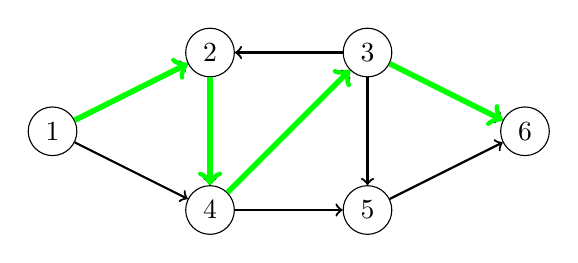
\begin{tikzpicture}
\node[draw, circle] (1) at (1,2) {$1$};
\node[draw, circle] (2) at (3,3) {$2$};
\node[draw, circle] (3) at (5,3) {$3$};
\node[draw, circle] (4) at (3,1) {$4$};
\node[draw, circle] (5) at (5,1) {$5$};
\node[draw, circle] (6) at (7,2) {$6$};
\path[draw,thick,->] (1) -- (2);
\path[draw,thick,->] (1) -- (4);
\path[draw,thick,->] (2) -- (4);
\path[draw,thick,->] (3) -- (2);
\path[draw,thick,->] (3) -- (5);
\path[draw,thick,->] (3) -- (6);
\path[draw,thick,->] (4) -- (3);
\path[draw,thick,->] (4) -- (5);
\path[draw,thick,->] (5) -- (6);

\path[draw=green,thick,->,line width=2pt] (1) -- (2);
\path[draw=green,thick,->,line width=2pt] (2) -- (4);
\path[draw=green,thick,->,line width=2pt] (4) -- (3);
\path[draw=green,thick,->,line width=2pt] (3) -- (6);
\end{tikzpicture}
\end{center}

Chúng ta cũng có thể quy bài toán này về bài toán luồng cực đại.
Vì mỗi nút có thể xuất hiện trong tối đa một đường đi,
chúng ta phải giới hạn luồng đi qua các nút.
Một phương pháp tiêu chuẩn cho việc này là chia mỗi nút thành
hai nút sao cho nút thứ nhất có các cạnh đi vào
của nút ban đầu, nút thứ hai có các cạnh đi ra
của nút ban đầu, và
có một cạnh mới từ nút thứ nhất
đến nút thứ hai.

Trong ví dụ của chúng ta, đồ thị trở thành như sau:
\begin{center}
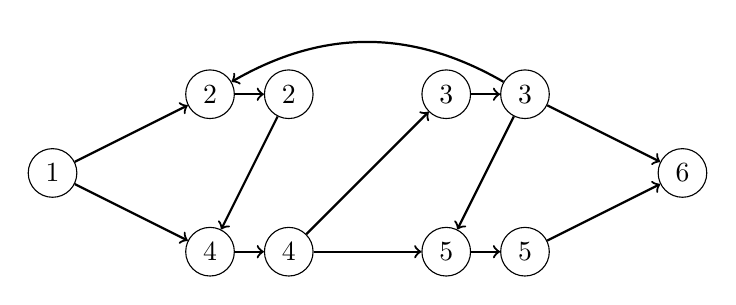
\begin{tikzpicture}
\node[draw, circle] (1) at (1,2) {$1$};

\node[draw, circle] (2a) at (3,3) {$2$};
\node[draw, circle] (3a) at (6,3) {$3$};
\node[draw, circle] (4a) at (3,1) {$4$};
\node[draw, circle] (5a) at (6,1) {$5$};

\node[draw, circle] (2b) at (4,3) {$2$};
\node[draw, circle] (3b) at (7,3) {$3$};
\node[draw, circle] (4b) at (4,1) {$4$};
\node[draw, circle] (5b) at (7,1) {$5$};

\node[draw, circle] (6) at (9,2) {$6$};

\path[draw,thick,->] (2a) -- (2b);
\path[draw,thick,->] (3a) -- (3b);
\path[draw,thick,->] (4a) -- (4b);
\path[draw,thick,->] (5a) -- (5b);

\path[draw,thick,->] (1) -- (2a);
\path[draw,thick,->] (1) -- (4a);
\path[draw,thick,->] (2b) -- (4a);
\path[draw,thick,->] (3b) edge [bend right=30] (2a);
\path[draw,thick,->] (3b) -- (5a);
\path[draw,thick,->] (3b) -- (6);
\path[draw,thick,->] (4b) -- (3a);
\path[draw,thick,->] (4b) -- (5a);
\path[draw,thick,->] (5b) -- (6);
\end{tikzpicture}
\end{center}

Luồng cực đại cho đồ thị là như sau:
\begin{center}
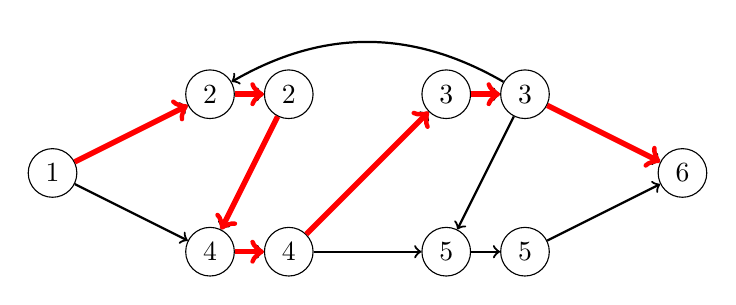
\begin{tikzpicture}
\node[draw, circle] (1) at (1,2) {$1$};

\node[draw, circle] (2a) at (3,3) {$2$};
\node[draw, circle] (3a) at (6,3) {$3$};
\node[draw, circle] (4a) at (3,1) {$4$};
\node[draw, circle] (5a) at (6,1) {$5$};

\node[draw, circle] (2b) at (4,3) {$2$};
\node[draw, circle] (3b) at (7,3) {$3$};
\node[draw, circle] (4b) at (4,1) {$4$};
\node[draw, circle] (5b) at (7,1) {$5$};

\node[draw, circle] (6) at (9,2) {$6$};

\path[draw,thick,->] (2a) -- (2b);
\path[draw,thick,->] (3a) -- (3b);
\path[draw,thick,->] (4a) -- (4b);
\path[draw,thick,->] (5a) -- (5b);

\path[draw,thick,->] (1) -- (2a);
\path[draw,thick,->] (1) -- (4a);
\path[draw,thick,->] (2b) -- (4a);
\path[draw,thick,->] (3b) edge [bend right=30] (2a);
\path[draw,thick,->] (3b) -- (5a);
\path[draw,thick,->] (3b) -- (6);
\path[draw,thick,->] (4b) -- (3a);
\path[draw,thick,->] (4b) -- (5a);
\path[draw,thick,->] (5b) -- (6);

\path[draw=red,thick,->,line width=2pt] (1) -- (2a);
\path[draw=red,thick,->,line width=2pt] (2a) -- (2b);
\path[draw=red,thick,->,line width=2pt] (2b) -- (4a);
\path[draw=red,thick,->,line width=2pt] (4a) -- (4b);
\path[draw=red,thick,->,line width=2pt] (4b) -- (3a);
\path[draw=red,thick,->,line width=2pt] (3a) -- (3b);
\path[draw=red,thick,->,line width=2pt] (3b) -- (6);
\end{tikzpicture}
\end{center}

Do đó, số lượng tối đa các đường đi không giao nhau trên đỉnh
từ nguồn đến đích là 1.

\section{Maximum matchings}

\index{matching}
\index{maximum matching}

Bài toán \key{maximum matching} yêu cầu tìm
một tập hợp các cặp nút có kích thước tối đa trong một đồ thị vô hướng
sao cho mỗi cặp được nối với nhau bằng một cạnh và
mỗi nút thuộc về tối đa một cặp.

Có các thuật toán đa thức để tìm
ghép cặp cực đại trong đồ thị tổng quát \cite{edm65},
nhưng các thuật toán như vậy rất phức tạp và
hiếm khi thấy trong các cuộc thi lập trình.
Tuy nhiên, trong các đồ thị hai phía,
bài toán ghép cặp cực đại dễ giải quyết hơn nhiều,
bởi vì chúng ta có thể quy nó về
bài toán luồng cực đại.

\subsubsection{Tìm ghép cặp cực đại}

Các nút của một đồ thị hai phía luôn có thể được
chia thành hai nhóm sao cho tất cả các cạnh
của đồ thị đi từ nhóm bên trái sang nhóm bên phải.
Ví dụ, trong đồ thị hai phía sau,
các nhóm là $\{1,2,3,4\}$ và $\{5,6,7,8\}$.

\begin{center}
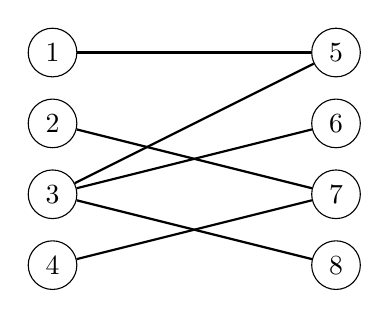
\begin{tikzpicture}[scale=0.60]
\node[draw, circle] (1) at (2,4.5) {1};
\node[draw, circle] (2) at (2,3) {2};
\node[draw, circle] (3) at (2,1.5) {3};
\node[draw, circle] (4) at (2,0) {4};
\node[draw, circle] (5) at (8,4.5) {5};
\node[draw, circle] (6) at (8,3) {6};
\node[draw, circle] (7) at (8,1.5) {7};
\node[draw, circle] (8) at (8,0) {8};

\path[draw,thick,-] (1) -- (5);
\path[draw,thick,-] (2) -- (7);
\path[draw,thick,-] (3) -- (5);
\path[draw,thick,-] (3) -- (6);
\path[draw,thick,-] (3) -- (8);
\path[draw,thick,-] (4) -- (7);
\end{tikzpicture}
\end{center}
Kích thước của một ghép cặp cực đại của đồ thị này là 3:
\begin{center}
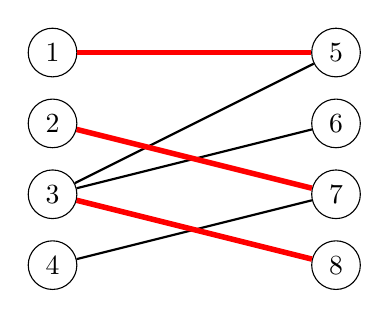
\begin{tikzpicture}[scale=0.60]
\node[draw, circle] (1) at (2,4.5) {1};
\node[draw, circle] (2) at (2,3) {2};
\node[draw, circle] (3) at (2,1.5) {3};
\node[draw, circle] (4) at (2,0) {4};
\node[draw, circle] (5) at (8,4.5) {5};
\node[draw, circle] (6) at (8,3) {6};
\node[draw, circle] (7) at (8,1.5) {7};
\node[draw, circle] (8) at (8,0) {8};

\path[draw,thick,-] (1) -- (5);
\path[draw,thick,-] (2) -- (7);
\path[draw,thick,-] (3) -- (5);
\path[draw,thick,-] (3) -- (6);
\path[draw,thick,-] (3) -- (8);
\path[draw,thick,-] (4) -- (7);

\path[draw=red,thick,-,line width=2pt] (1) -- (5);
\path[draw=red,thick,-,line width=2pt] (2) -- (7);
\path[draw=red,thick,-,line width=2pt] (3) -- (8);
\end{tikzpicture}
\end{center}

Chúng ta có thể quy bài toán ghép cặp cực đại trên đồ thị hai phía
về bài toán luồng cực đại bằng cách thêm hai nút mới
vào đồ thị: một nguồn và một đích.
Chúng ta cũng thêm các cạnh từ nguồn
đến mỗi nút bên trái và từ mỗi nút bên phải đến đích.
Sau đó, kích thước của một luồng cực đại trong đồ thị
bằng kích thước của một ghép cặp cực đại trong đồ thị ban đầu.

Ví dụ, việc quy đổi cho đồ thị trên
như sau:
\begin{center}
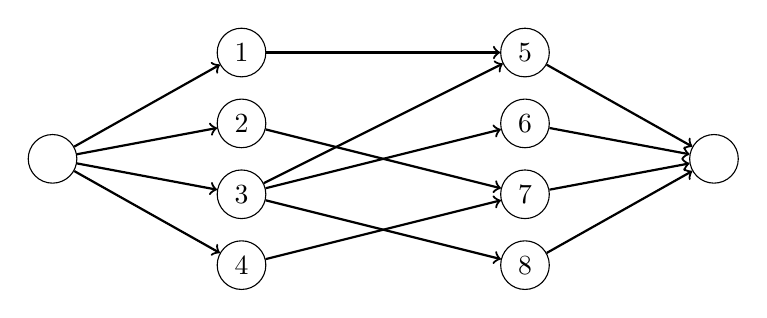
\begin{tikzpicture}[scale=0.60]
\node[draw, circle] (1) at (2,4.5) {1};
\node[draw, circle] (2) at (2,3) {2};
\node[draw, circle] (3) at (2,1.5) {3};
\node[draw, circle] (4) at (2,0) {4};
\node[draw, circle] (5) at (8,4.5) {5};
\node[draw, circle] (6) at (8,3) {6};
\node[draw, circle] (7) at (8,1.5) {7};
\node[draw, circle] (8) at (8,0) {8};

\node[draw, circle] (a) at (-2,2.25) {\phantom{0}};
\node[draw, circle] (b) at (12,2.25) {\phantom{0}};

\path[draw,thick,->] (1) -- (5);
\path[draw,thick,->] (2) -- (7);
\path[draw,thick,->] (3) -- (5);
\path[draw,thick,->] (3) -- (6);
\path[draw,thick,->] (3) -- (8);
\path[draw,thick,->] (4) -- (7);

\path[draw,thick,->] (a) -- (1);
\path[draw,thick,->] (a) -- (2);
\path[draw,thick,->] (a) -- (3);
\path[draw,thick,->] (a) -- (4);
\path[draw,thick,->] (5) -- (b);
\path[draw,thick,->] (6) -- (b);
\path[draw,thick,->] (7) -- (b);
\path[draw,thick,->] (8) -- (b);
\end{tikzpicture}
\end{center}

Luồng cực đại của đồ thị này như sau:
\begin{center}
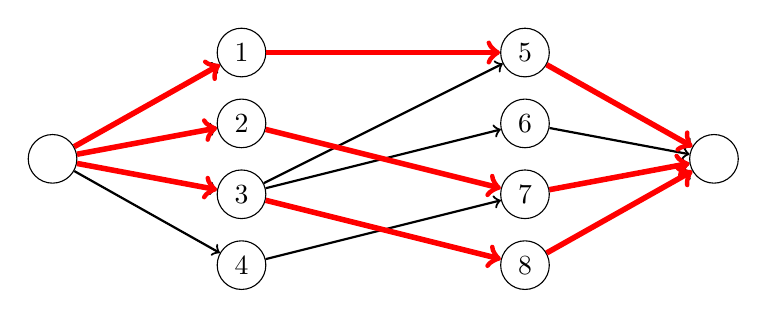
\begin{tikzpicture}[scale=0.60]
\node[draw, circle] (1) at (2,4.5) {1};
\node[draw, circle] (2) at (2,3) {2};
\node[draw, circle] (3) at (2,1.5) {3};
\node[draw, circle] (4) at (2,0) {4};
\node[draw, circle] (5) at (8,4.5) {5};
\node[draw, circle] (6) at (8,3) {6};
\node[draw, circle] (7) at (8,1.5) {7};
\node[draw, circle] (8) at (8,0) {8};

\node[draw, circle] (a) at (-2,2.25) {\phantom{0}};
\node[draw, circle] (b) at (12,2.25) {\phantom{0}};

\path[draw,thick,->] (3) -- (5);
\path[draw,thick,->] (3) -- (6);
\path[draw,thick,->] (4) -- (7);

\path[draw,thick,->] (a) -- (1);
\path[draw,thick,->] (a) -- (2);
\path[draw,thick,->] (a) -- (3);
\path[draw,thick,->] (a) -- (4);
\path[draw,thick,->] (5) -- (b);
\path[draw,thick,->] (6) -- (b);
\path[draw,thick,->] (7) -- (b);
\path[draw,thick,->] (8) -- (b);

\path[draw=red,thick,->,line width=2pt] (1) -- (5);
\path[draw=red,thick,->,line width=2pt] (2) -- (7);
\path[draw=red,thick,->,line width=2pt] (3) -- (8);

\path[draw=red,thick,->,line width=2pt] (a) -- (1);
\path[draw=red,thick,->,line width=2pt] (a) -- (2);
\path[draw=red,thick,->,line width=2pt] (a) -- (3);

\path[draw=red,thick,->,line width=2pt] (5) -- (b);
\path[draw=red,thick,->,line width=2pt] (7) -- (b);
\path[draw=red,thick,->,line width=2pt] (8) -- (b);

\end{tikzpicture}
\end{center}

\subsubsection{Hall's theorem}

\index{Hall's theorem}
\index{perfect matching}

\key{Định lý Hall (Hall's theorem)} có thể được sử dụng để tìm ra
liệu một đồ thị hai phía có một ghép cặp
chứa tất cả các nút bên trái hoặc bên phải hay không.
Nếu số lượng nút bên trái và bên phải bằng nhau,
định lý Hall cho chúng ta biết liệu có thể
xây dựng một \key{ghép cặp hoàn hảo (perfect matching)}
chứa tất cả các nút của đồ thị hay không.

Giả sử chúng ta muốn tìm một ghép cặp
chứa tất cả các nút bên trái.
Gọi $X$ là một tập hợp bất kỳ các nút bên trái
và gọi $f(X)$ là tập hợp các hàng xóm của chúng.
Theo định lý Hall, một ghép cặp
chứa tất cả các nút bên trái tồn tại
chính xác khi với mỗi $X$, điều kiện $|X| \le |f(X)|$ thỏa mãn.

Hãy nghiên cứu định lý Hall trong đồ thị ví dụ.
Đầu tiên, đặt $X=\{1,3\}$, ta có $f(X)=\{5,6,8\}$:

\begin{center}
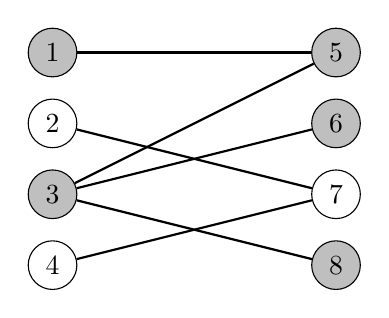
\begin{tikzpicture}[scale=0.60]
\node[draw, circle, fill=lightgray] (1) at (2,4.5) {1};
\node[draw, circle] (2) at (2,3) {2};
\node[draw, circle, fill=lightgray] (3) at (2,1.5) {3};
\node[draw, circle] (4) at (2,0) {4};
\node[draw, circle, fill=lightgray] (5) at (8,4.5) {5};
\node[draw, circle, fill=lightgray] (6) at (8,3) {6};
\node[draw, circle] (7) at (8,1.5) {7};
\node[draw, circle, fill=lightgray] (8) at (8,0) {8};

\path[draw,thick,-] (1) -- (5);
\path[draw,thick,-] (2) -- (7);
\path[draw,thick,-] (3) -- (5);
\path[draw,thick,-] (3) -- (6);
\path[draw,thick,-] (3) -- (8);
\path[draw,thick,-] (4) -- (7);
\end{tikzpicture}
\end{center}

Điều kiện của định lý Hall thỏa mãn, bởi vì
$|X|=2$ và $|f(X)|=3$.
Tiếp theo, đặt $X=\{2,4\}$, ta có $f(X)=\{7\}$:

\begin{center}
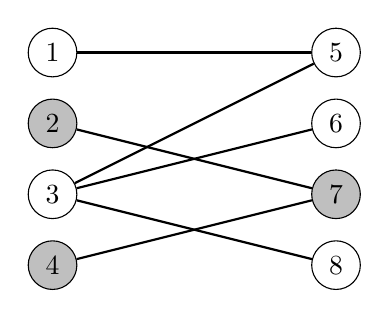
\begin{tikzpicture}[scale=0.60]
\node[draw, circle] (1) at (2,4.5) {1};
\node[draw, circle, fill=lightgray] (2) at (2,3) {2};
\node[draw, circle] (3) at (2,1.5) {3};
\node[draw, circle, fill=lightgray] (4) at (2,0) {4};
\node[draw, circle] (5) at (8,4.5) {5};
\node[draw, circle] (6) at (8,3) {6};
\node[draw, circle, fill=lightgray] (7) at (8,1.5) {7};
\node[draw, circle] (8) at (8,0) {8};

\path[draw,thick,-] (1) -- (5);
\path[draw,thick,-] (2) -- (7);
\path[draw,thick,-] (3) -- (5);
\path[draw,thick,-] (3) -- (6);
\path[draw,thick,-] (3) -- (8);
\path[draw,thick,-] (4) -- (7);
\end{tikzpicture}
\end{center}

Trong trường hợp này, $|X|=2$ và $|f(X)|=1$,
vì vậy điều kiện của định lý Hall không thỏa mãn.
Điều này có nghĩa là không thể tạo thành
một ghép cặp hoàn hảo cho đồ thị.
Kết quả này không đáng ngạc nhiên, bởi vì chúng ta đã
biết rằng ghép cặp cực đại của đồ thị là 3 chứ không phải 4.

Nếu điều kiện của định lý Hall không thỏa mãn,
tập hợp $X$ cung cấp một lời giải thích \emph{tại sao}
chúng ta không thể tạo thành một ghép cặp như vậy.
Vì $X$ chứa nhiều nút hơn $f(X)$,
không có đủ cặp cho tất cả các nút trong $X$.
Ví dụ, trong đồ thị trên, cả hai nút 2 và 4
đều phải được nối với nút 7, điều này là không thể.

\subsubsection{Kőnig's theorem}

\index{Kőnig's theorem}
\index{node cover}
\index{minimum node cover}

Một \key{phủ đỉnh tối thiểu (minimum node cover)} của một đồ thị
là một tập hợp các nút có kích thước tối thiểu sao cho mỗi cạnh của đồ thị
có ít nhất một điểm cuối trong tập hợp.
Trong một đồ thị tổng quát, việc tìm một phủ đỉnh tối thiểu
là một bài toán NP-khó.
Tuy nhiên, nếu đồ thị là hai phía,
\key{Định lý Kőnig (Kőnig's theorem)} cho chúng ta biết rằng
kích thước của một phủ đỉnh tối thiểu
và kích thước của một ghép cặp cực đại luôn bằng nhau.
Do đó, chúng ta có thể tính kích thước của một phủ đỉnh tối thiểu
bằng cách sử dụng một thuật toán luồng cực đại.

Hãy xem xét đồ thị sau
với một ghép cặp cực đại có kích thước 3:
\begin{center}
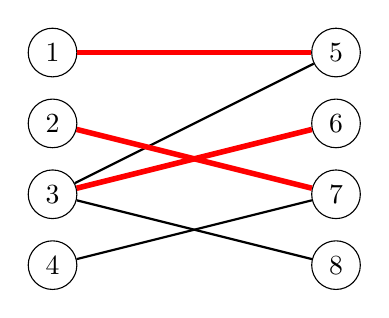
\begin{tikzpicture}[scale=0.60]
\node[draw, circle] (1) at (2,4.5) {1};
\node[draw, circle] (2) at (2,3) {2};
\node[draw, circle] (3) at (2,1.5) {3};
\node[draw, circle] (4) at (2,0) {4};
\node[draw, circle] (5) at (8,4.5) {5};
\node[draw, circle] (6) at (8,3) {6};
\node[draw, circle] (7) at (8,1.5) {7};
\node[draw, circle] (8) at (8,0) {8};

\path[draw,thick,-] (1) -- (5);
\path[draw,thick,-] (2) -- (7);
\path[draw,thick,-] (3) -- (5);
\path[draw,thick,-] (3) -- (6);
\path[draw,thick,-] (3) -- (8);
\path[draw,thick,-] (4) -- (7);

\path[draw=red,thick,-,line width=2pt] (1) -- (5);
\path[draw=red,thick,-,line width=2pt] (2) -- (7);
\path[draw=red,thick,-,line width=2pt] (3) -- (6);
\end{tikzpicture}
\end{center}
Bây giờ định lý Kőnig cho chúng ta biết rằng kích thước
của một phủ đỉnh tối thiểu cũng là 3.
Một phủ như vậy có thể được xây dựng như sau:

\begin{center}
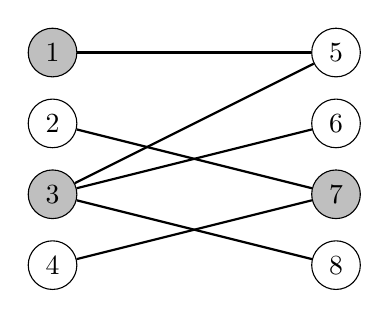
\begin{tikzpicture}[scale=0.60]
\node[draw, circle, fill=lightgray] (1) at (2,4.5) {1};
\node[draw, circle] (2) at (2,3) {2};
\node[draw, circle, fill=lightgray] (3) at (2,1.5) {3};
\node[draw, circle] (4) at (2,0) {4};
\node[draw, circle] (5) at (8,4.5) {5};
\node[draw, circle] (6) at (8,3) {6};
\node[draw, circle, fill=lightgray] (7) at (8,1.5) {7};
\node[draw, circle] (8) at (8,0) {8};

\path[draw,thick,-] (1) -- (5);
\path[draw,thick,-] (2) -- (7);
\path[draw,thick,-] (3) -- (5);
\path[draw,thick,-] (3) -- (6);
\path[draw,thick,-] (3) -- (8);
\path[draw,thick,-] (4) -- (7);
\end{tikzpicture}
\end{center}

\index{independent set}
\index{maximum independent set}

Các nút \emph{không}
thuộc về một phủ đỉnh tối thiểu
tạo thành một \key{tập độc lập cực đại (maximum independent set)}.
Đây là tập hợp các nút lớn nhất có thể
sao cho không có hai nút nào trong tập hợp
được nối với nhau bằng một cạnh.
Một lần nữa, việc tìm một tập độc lập cực đại
trong một đồ thị tổng quát là một bài toán NP-khó,
nhưng trong một đồ thị hai phía, chúng ta có thể sử dụng
định lý Kőnig để giải quyết bài toán một cách hiệu quả.
Trong đồ thị ví dụ, tập độc lập cực đại
như sau:

\begin{center}
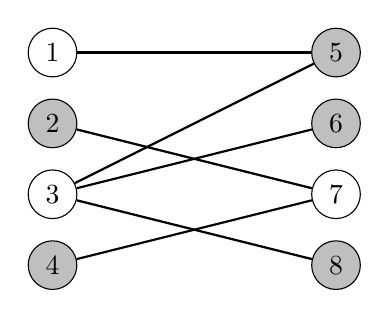
\begin{tikzpicture}[scale=0.60]
\node[draw, circle] (1) at (2,4.5) {1};
\node[draw, circle, fill=lightgray] (2) at (2,3) {2};
\node[draw, circle] (3) at (2,1.5) {3};
\node[draw, circle, fill=lightgray] (4) at (2,0) {4};
\node[draw, circle, fill=lightgray] (5) at (8,4.5) {5};
\node[draw, circle, fill=lightgray] (6) at (8,3) {6};
\node[draw, circle] (7) at (8,1.5) {7};
\node[draw, circle, fill=lightgray] (8) at (8,0) {8};

\path[draw,thick,-] (1) -- (5);
\path[draw,thick,-] (2) -- (7);
\path[draw,thick,-] (3) -- (5);
\path[draw,thick,-] (3) -- (6);
\path[draw,thick,-] (3) -- (8);
\path[draw,thick,-] (4) -- (7);
\end{tikzpicture}
\end{center}

\section{Path covers}

\index{path cover}

Một \key{phủ đường đi (path cover)} là một tập hợp các đường đi trong một đồ thị
sao cho mỗi nút của đồ thị thuộc về ít nhất một đường đi.
Hóa ra trong các đồ thị có hướng, không chu trình,
chúng ta có thể quy bài toán tìm một
phủ đường đi tối thiểu về bài toán tìm một luồng cực đại
trong một đồ thị khác.

\subsubsection{Node-disjoint path cover}

Trong một \key{phủ đường đi không giao nhau trên đỉnh (node-disjoint path cover)},
mỗi nút thuộc về chính xác một đường đi.
Ví dụ, hãy xem xét đồ thị sau:
\begin{center}
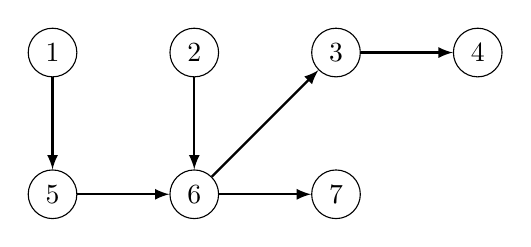
\begin{tikzpicture}[scale=0.9]
\node[draw, circle] (1) at (0,0) {1};
\node[draw, circle] (2) at (2,0) {2};
\node[draw, circle] (3) at (4,0) {3};
\node[draw, circle] (4) at (6,0) {4};
\node[draw, circle] (5) at (0,-2) {5};
\node[draw, circle] (6) at (2,-2) {6};
\node[draw, circle] (7) at (4,-2) {7};

\path[draw,thick,->,>=latex] (1) -- (5);
\path[draw,thick,->,>=latex] (2) -- (6);
\path[draw,thick,->,>=latex] (3) -- (4);
\path[draw,thick,->,>=latex] (5) -- (6);
\path[draw,thick,->,>=latex] (6) -- (3);
\path[draw,thick,->,>=latex] (6) -- (7);
\end{tikzpicture}
\end{center}

Một phủ đường đi không giao nhau trên đỉnh tối thiểu
của đồ thị này
bao gồm ba đường đi.
Ví dụ, chúng ta có thể chọn các đường đi sau:

\begin{center}
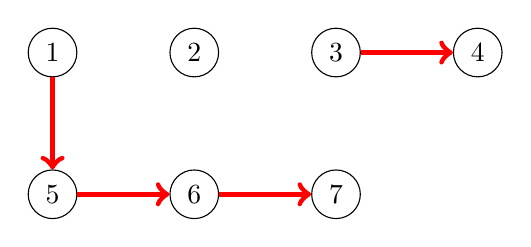
\begin{tikzpicture}[scale=0.9]
\node[draw, circle] (1) at (0,0) {1};
\node[draw, circle] (2) at (2,0) {2};
\node[draw, circle] (3) at (4,0) {3};
\node[draw, circle] (4) at (6,0) {4};
\node[draw, circle] (5) at (0,-2) {5};
\node[draw, circle] (6) at (2,-2) {6};
\node[draw, circle] (7) at (4,-2) {7};

\path[draw=red,thick,->,line width=2pt] (1) -- (5);
\path[draw=red,thick,->,line width=2pt] (5) -- (6);
\path[draw=red,thick,->,line width=2pt] (6) -- (7);
\path[draw=red,thick,->,line width=2pt] (3) -- (4);
\end{tikzpicture}
\end{center}

Lưu ý rằng một trong các đường đi chỉ chứa nút 2,
vì vậy có thể một đường đi không chứa bất kỳ cạnh nào.

Chúng ta có thể tìm một phủ đường đi không giao nhau trên đỉnh tối thiểu
bằng cách xây dựng một \emph{đồ thị ghép cặp} trong đó mỗi nút
của đồ thị ban đầu được biểu diễn bởi
hai nút: một nút bên trái và một nút bên phải.
Có một cạnh từ một nút bên trái đến một nút bên phải
nếu có một cạnh như vậy trong đồ thị ban đầu.
Ngoài ra, đồ thị ghép cặp chứa một nguồn và một đích,
và có các cạnh từ nguồn đến tất cả
các nút bên trái và từ tất cả các nút bên phải đến đích.

Một ghép cặp cực đại trong đồ thị kết quả tương ứng
với một phủ đường đi không giao nhau trên đỉnh tối thiểu trong
đồ thị ban đầu.
Ví dụ, đồ thị ghép cặp sau
cho đồ thị trên chứa
một ghép cặp cực đại có kích thước 4:

\begin{center}
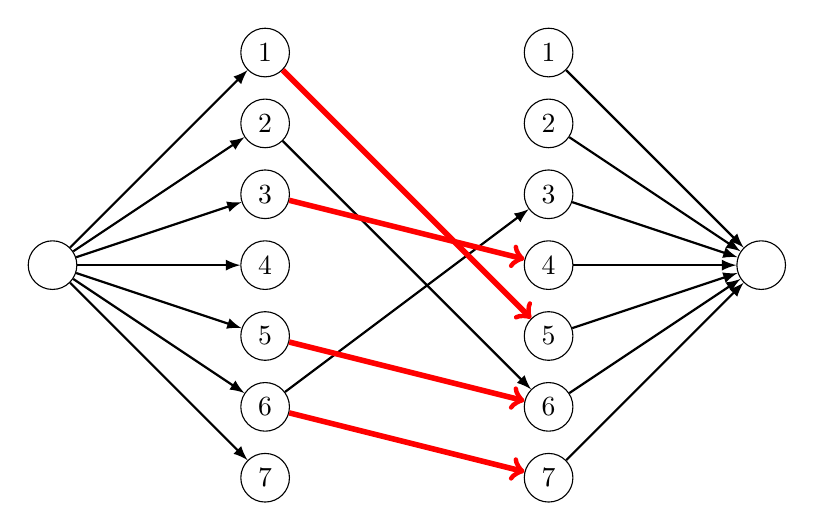
\begin{tikzpicture}[scale=0.9]
\node[draw, circle] (1a) at (0,6) {1};
\node[draw, circle] (2a) at (0,5) {2};
\node[draw, circle] (3a) at (0,4) {3};
\node[draw, circle] (4a) at (0,3) {4};
\node[draw, circle] (5a) at (0,2) {5};
\node[draw, circle] (6a) at (0,1) {6};
\node[draw, circle] (7a) at (0,0) {7};

\node[draw, circle] (1b) at (4,6) {1};
\node[draw, circle] (2b) at (4,5) {2};
\node[draw, circle] (3b) at (4,4) {3};
\node[draw, circle] (4b) at (4,3) {4};
\node[draw, circle] (5b) at (4,2) {5};
\node[draw, circle] (6b) at (4,1) {6};
\node[draw, circle] (7b) at (4,0) {7};

\node[draw, circle] (a) at (-3,3) {\phantom{0}};
\node[draw, circle] (b) at (7,3) {\phantom{0}};

%\path[draw,thick,->,>=latex] (1a) -- (5b);
\path[draw,thick,->,>=latex] (2a) -- (6b);
%\path[draw,thick,->,>=latex] (3a) -- (4b);
%\path[draw,thick,->,>=latex] (5a) -- (6b);
\path[draw,thick,->,>=latex] (6a) -- (3b);
%\path[draw,thick,->,>=latex] (6a) -- (7b);

\path[draw,thick,->,>=latex] (a) -- (1a);
\path[draw,thick,->,>=latex] (a) -- (2a);
\path[draw,thick,->,>=latex] (a) -- (3a);
\path[draw,thick,->,>=latex] (a) -- (4a);
\path[draw,thick,->,>=latex] (a) -- (5a);
\path[draw,thick,->,>=latex] (a) -- (6a);
\path[draw,thick,->,>=latex] (a) -- (7a);

\path[draw,thick,->,>=latex] (1b) -- (b);
\path[draw,thick,->,>=latex] (2b) -- (b);
\path[draw,thick,->,>=latex] (3b) -- (b);
\path[draw,thick,->,>=latex] (4b) -- (b);
\path[draw,thick,->,>=latex] (5b) -- (b);
\path[draw,thick,->,>=latex] (6b) -- (b);
\path[draw,thick,->,>=latex] (7b) -- (b);

\path[draw=red,thick,->,line width=2pt] (1a) -- (5b);
\path[draw=red,thick,->,line width=2pt] (5a) -- (6b);
\path[draw=red,thick,->,line width=2pt] (6a) -- (7b);
\path[draw=red,thick,->,line width=2pt] (3a) -- (4b);

\end{tikzpicture}
\end{center}

Mỗi cạnh trong ghép cặp cực đại của đồ thị ghép cặp tương ứng
với một cạnh trong phủ đường đi không giao nhau trên đỉnh tối thiểu
của đồ thị ban đầu.
Do đó, kích thước của phủ đường đi không giao nhau trên đỉnh tối thiểu là $n-c$,
trong đó $n$ là số nút trong đồ thị ban đầu
và $c$ là kích thước của ghép cặp cực đại.

\subsubsection{General path cover}

Một \key{phủ đường đi tổng quát (general path cover)} là một phủ đường đi
trong đó một nút có thể thuộc về nhiều hơn một đường đi.
Một phủ đường đi tổng quát tối thiểu có thể nhỏ hơn
một phủ đường đi không giao nhau trên đỉnh tối thiểu,
bởi vì một nút có thể được sử dụng nhiều lần trong các đường đi.
Hãy xem xét lại đồ thị sau:
\begin{center}
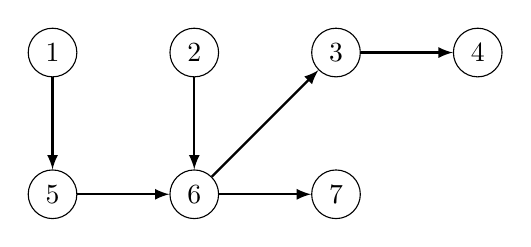
\begin{tikzpicture}[scale=0.9]
\node[draw, circle] (1) at (0,0) {1};
\node[draw, circle] (2) at (2,0) {2};
\node[draw, circle] (3) at (4,0) {3};
\node[draw, circle] (4) at (6,0) {4};
\node[draw, circle] (5) at (0,-2) {5};
\node[draw, circle] (6) at (2,-2) {6};
\node[draw, circle] (7) at (4,-2) {7};

\path[draw,thick,->,>=latex] (1) -- (5);
\path[draw,thick,->,>=latex] (2) -- (6);
\path[draw,thick,->,>=latex] (3) -- (4);
\path[draw,thick,->,>=latex] (5) -- (6);
\path[draw,thick,->,>=latex] (6) -- (3);
\path[draw,thick,->,>=latex] (6) -- (7);
\end{tikzpicture}
\end{center}

Phủ đường đi tổng quát tối thiểu của đồ thị này
bao gồm hai đường đi.
Ví dụ, đường đi thứ nhất có thể như sau:
\begin{center}
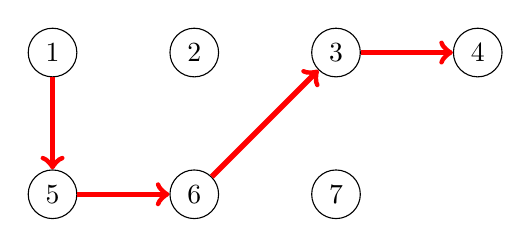
\begin{tikzpicture}[scale=0.9]
\node[draw, circle] (1) at (0,0) {1};
\node[draw, circle] (2) at (2,0) {2};
\node[draw, circle] (3) at (4,0) {3};
\node[draw, circle] (4) at (6,0) {4};
\node[draw, circle] (5) at (0,-2) {5};
\node[draw, circle] (6) at (2,-2) {6};
\node[draw, circle] (7) at (4,-2) {7};

\path[draw=red,thick,->,line width=2pt] (1) -- (5);
\path[draw=red,thick,->,line width=2pt] (5) -- (6);
\path[draw=red,thick,->,line width=2pt] (6) -- (3);
\path[draw=red,thick,->,line width=2pt] (3) -- (4);
\end{tikzpicture}
\end{center}
Và đường đi thứ hai có thể như sau:
\begin{center}
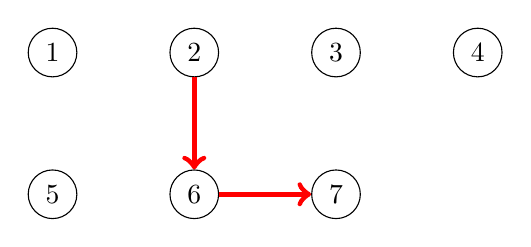
\begin{tikzpicture}[scale=0.9]
\node[draw, circle] (1) at (0,0) {1};
\node[draw, circle] (2) at (2,0) {2};
\node[draw, circle] (3) at (4,0) {3};
\node[draw, circle] (4) at (6,0) {4};
\node[draw, circle] (5) at (0,-2) {5};
\node[draw, circle] (6) at (2,-2) {6};
\node[draw, circle] (7) at (4,-2) {7};

\path[draw=red,thick,->,line width=2pt] (2) -- (6);
\path[draw=red,thick,->,line width=2pt] (6) -- (7);
\end{tikzpicture}
\end{center}

Một phủ đường đi tổng quát tối thiểu có thể được tìm thấy
gần giống như một phủ đường đi không giao nhau trên đỉnh tối thiểu.
Chỉ cần thêm một số cạnh mới vào đồ thị ghép cặp
sao cho luôn có một cạnh $a \rightarrow b$
bất cứ khi nào có một đường đi từ $a$ đến $b$
trong đồ thị ban đầu (có thể qua nhiều cạnh).

Đồ thị ghép cặp cho đồ thị trên như sau:
\begin{center}
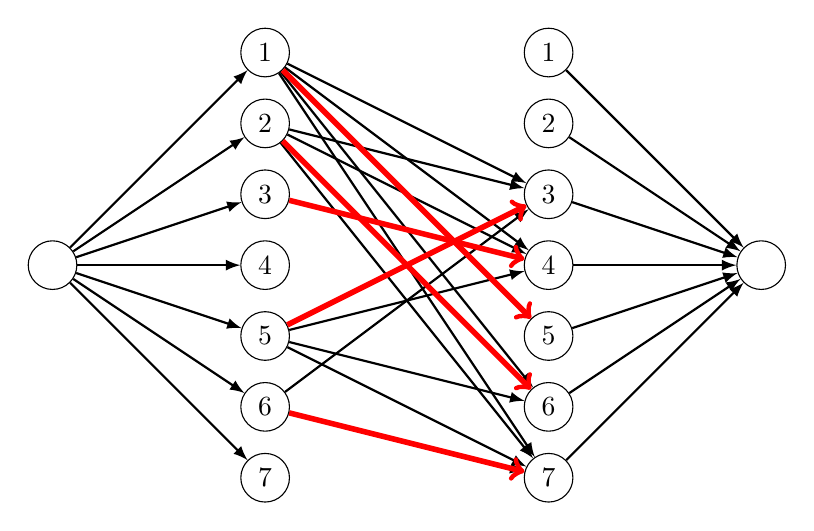
\begin{tikzpicture}[scale=0.9]
\node[draw, circle] (1a) at (0,6) {1};
\node[draw, circle] (2a) at (0,5) {2};
\node[draw, circle] (3a) at (0,4) {3};
\node[draw, circle] (4a) at (0,3) {4};
\node[draw, circle] (5a) at (0,2) {5};
\node[draw, circle] (6a) at (0,1) {6};
\node[draw, circle] (7a) at (0,0) {7};

\node[draw, circle] (1b) at (4,6) {1};
\node[draw, circle] (2b) at (4,5) {2};
\node[draw, circle] (3b) at (4,4) {3};
\node[draw, circle] (4b) at (4,3) {4};
\node[draw, circle] (5b) at (4,2) {5};
\node[draw, circle] (6b) at (4,1) {6};
\node[draw, circle] (7b) at (4,0) {7};

\node[draw, circle] (a) at (-3,3) {\phantom{0}};
\node[draw, circle] (b) at (7,3) {\phantom{0}};


%\path[draw,thick,->,>=latex] (1a) -- (5b);
\path[draw,thick,->,>=latex] (1a) -- (6b);
\path[draw,thick,->,>=latex] (1a) -- (7b);
\path[draw,thick,->,>=latex] (1a) -- (3b);
\path[draw,thick,->,>=latex] (1a) -- (4b);
\path[draw,thick,->,>=latex] (5a) -- (6b);
\path[draw,thick,->,>=latex] (5a) -- (7b);
%\path[draw,thick,->,>=latex] (5a) -- (3b);
\path[draw,thick,->,>=latex] (5a) -- (4b);
\path[draw,thick,->,>=latex] (6a) -- (7b);
%\path[draw,thick,->,>=latex] (6a) -- (7b);
\path[draw,thick,->,>=latex] (6a) -- (3b);
%\path[draw,thick,->,>=latex] (3a) -- (4b);
%\path[draw,thick,->,>=latex] (2a) -- (6b);
\path[draw,thick,->,>=latex] (2a) -- (7b);
\path[draw,thick,->,>=latex] (2a) -- (3b);
\path[draw,thick,->,>=latex] (2a) -- (4b);


\path[draw,thick,->,>=latex] (a) -- (1a);
\path[draw,thick,->,>=latex] (a) -- (2a);
\path[draw,thick,->,>=latex] (a) -- (3a);
\path[draw,thick,->,>=latex] (a) -- (4a);
\path[draw,thick,->,>=latex] (a) -- (5a);
\path[draw,thick,->,>=latex] (a) -- (6a);
\path[draw,thick,->,>=latex] (a) -- (7a);

\path[draw,thick,->,>=latex] (1b) -- (b);
\path[draw,thick,->,>=latex] (2b) -- (b);
\path[draw,thick,->,>=latex] (3b) -- (b);
\path[draw,thick,->,>=latex] (4b) -- (b);
\path[draw,thick,->,>=latex] (5b) -- (b);
\path[draw,thick,->,>=latex] (6b) -- (b);
\path[draw,thick,->,>=latex] (7b) -- (b);

\path[draw=red,thick,->,line width=2pt] (1a) -- (5b);
\path[draw=red,thick,->,line width=2pt] (5a) -- (3b);
\path[draw=red,thick,->,line width=2pt] (3a) -- (4b);
\path[draw=red,thick,->,line width=2pt] (2a) -- (6b);
\path[draw=red,thick,->,line width=2pt] (6a) -- (7b);

\end{tikzpicture}
\end{center}

\subsubsection{Dilworth's theorem}

\index{Dilworth's theorem}
\index{antichain}

Một \key{đối chuỗi (antichain)} là một tập hợp các nút của một đồ thị
sao cho không có đường đi
từ bất kỳ nút nào đến một nút khác
sử dụng các cạnh của đồ thị.
\key{Định lý Dilworth (Dilworth's theorem)} phát biểu rằng
trong một đồ thị có hướng không chu trình, kích thước của
một phủ đường đi tổng quát tối thiểu
bằng kích thước của một đối chuỗi cực đại.

Ví dụ, các nút 3 và 7 tạo thành một đối chuỗi
trong đồ thị sau:

\begin{center}
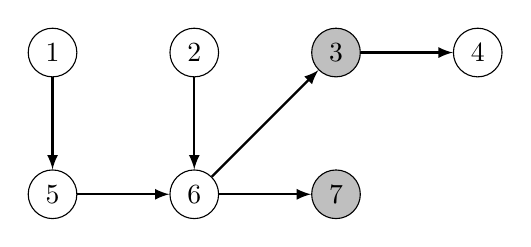
\begin{tikzpicture}[scale=0.9]
\node[draw, circle] (1) at (0,0) {1};
\node[draw, circle] (2) at (2,0) {2};
\node[draw, circle, fill=lightgray] (3) at (4,0) {3};
\node[draw, circle] (4) at (6,0) {4};
\node[draw, circle] (5) at (0,-2) {5};
\node[draw, circle] (6) at (2,-2) {6};
\node[draw, circle, fill=lightgray] (7) at (4,-2) {7};

\path[draw,thick,->,>=latex] (1) -- (5);
\path[draw,thick,->,>=latex] (2) -- (6);
\path[draw,thick,->,>=latex] (3) -- (4);
\path[draw,thick,->,>=latex] (5) -- (6);
\path[draw,thick,->,>=latex] (6) -- (3);
\path[draw,thick,->,>=latex] (6) -- (7);
\end{tikzpicture}
\end{center}

Đây là một đối chuỗi cực đại, vì không thể
xây dựng bất kỳ đối chuỗi nào chứa ba nút.
Chúng ta đã thấy trước đó rằng kích thước của một phủ
đường đi tổng quát tối thiểu của đồ thị này bao gồm hai đường đi.